\documentclass{standalone}
\usepackage{tikz}
\usetikzlibrary{patterns, positioning}
\usepackage[sfdefault]{ClearSans} %% option 'sfdefault' activates Clear Sans as the default text font
\usepackage[T1]{fontenc}

\begin{document}
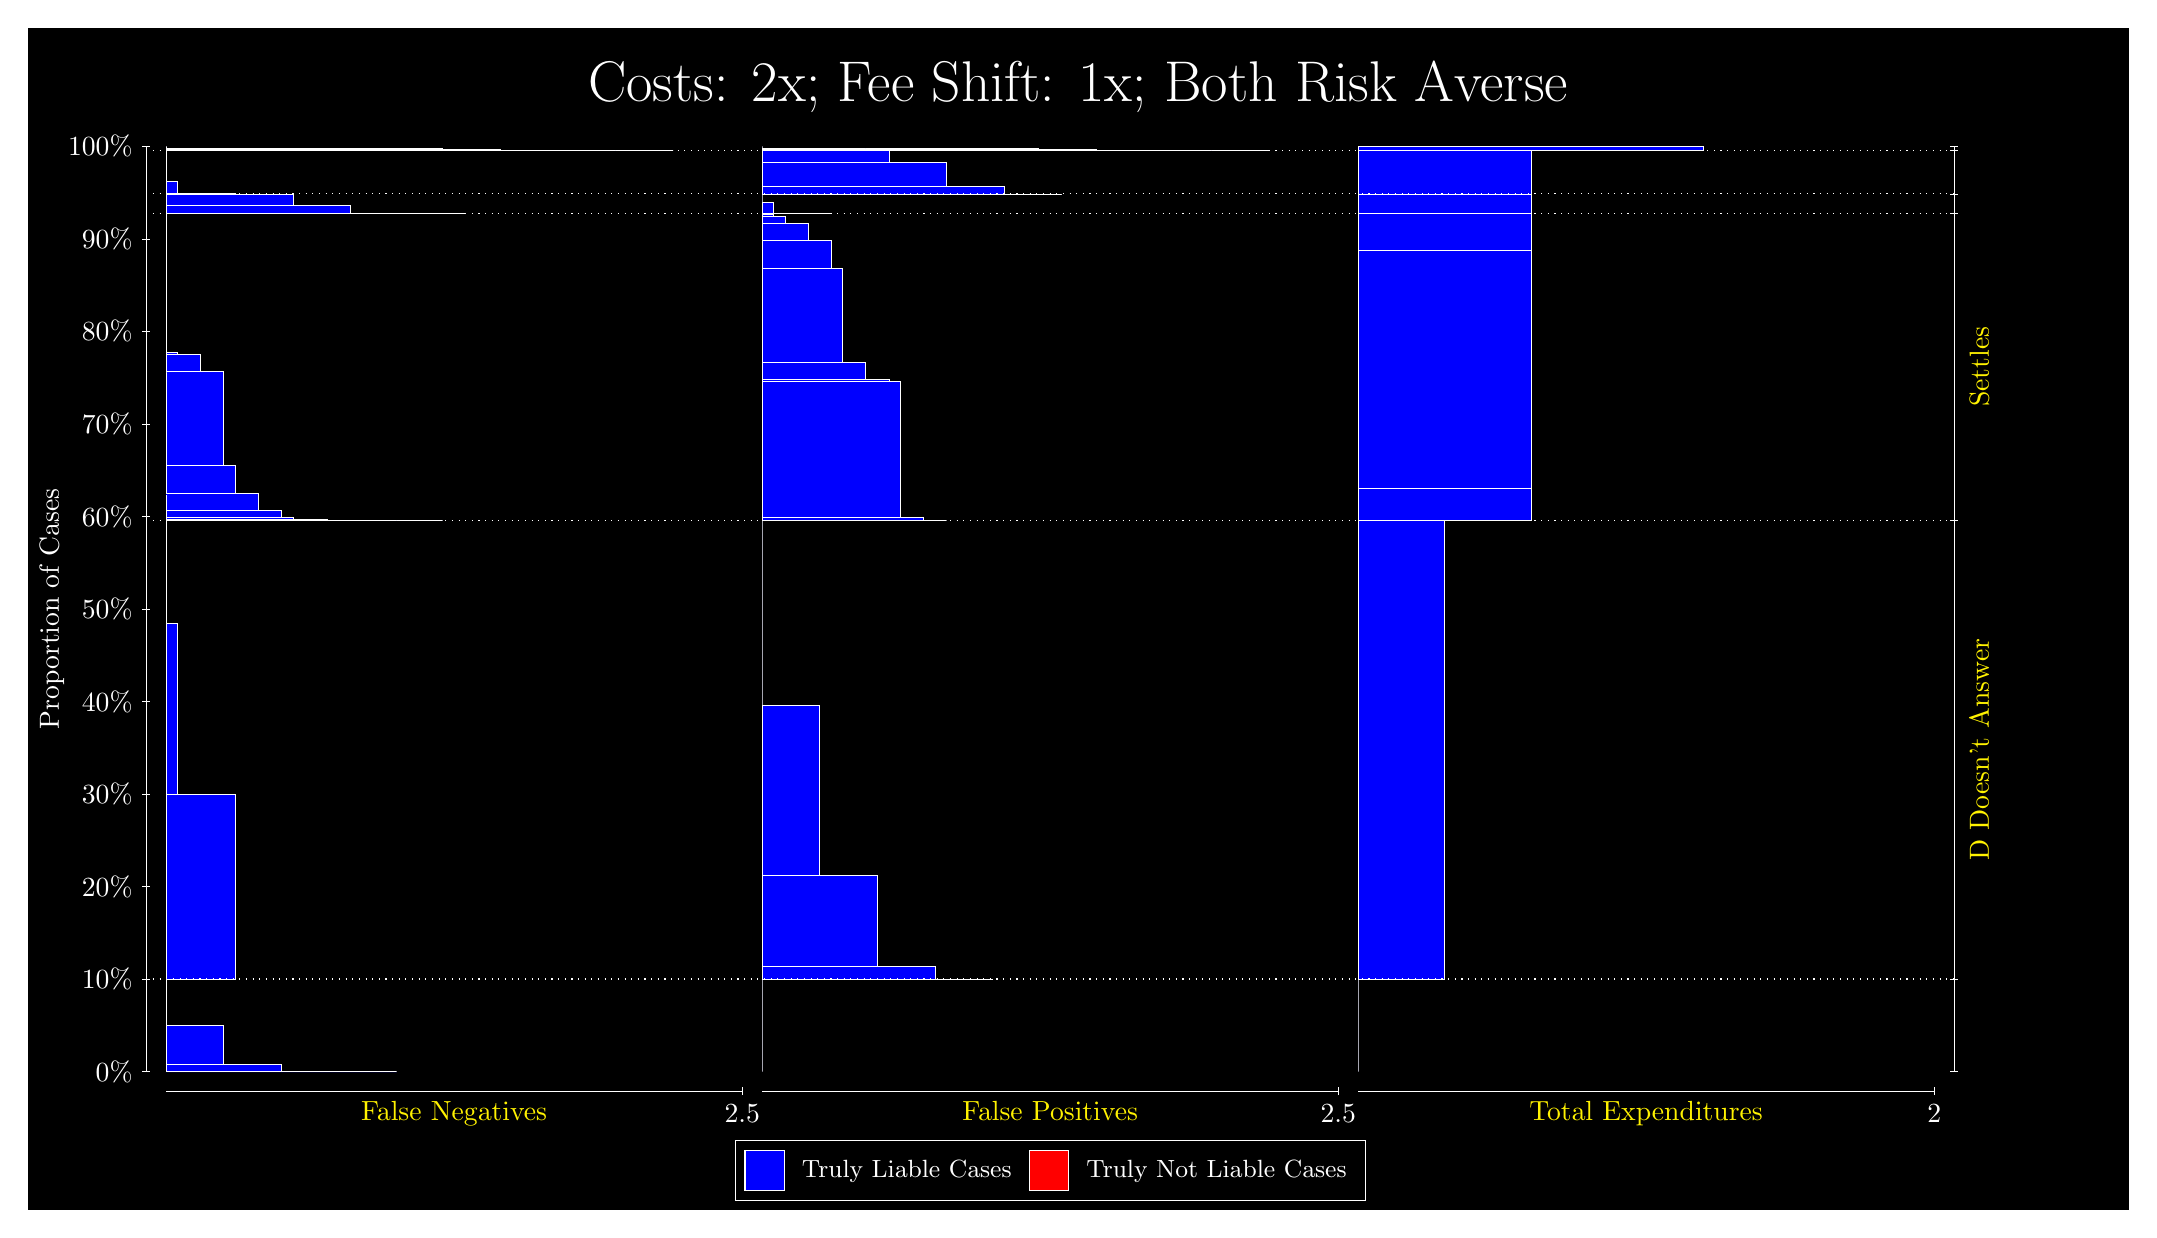
\begin{tikzpicture}
\draw[fill=black] (0,0) rectangle (26.667,15);
\draw[text=white] (0,13.5) rectangle (26.667,15) node[midway] {\huge Costs: 2x; Fee Shift: 1x; Both Risk Averse};
\draw[white, very thin] (1.5,1.75) -- (1.5,13.5);
\node[rotate=90, text=white, anchor=center] at (0.3, 7.625) {Proportion of Cases};
\draw[white, very thin] (1.45,1.75) -- (1.55,1.75);
\node[text=white, anchor=east] at (1.45, 1.75) {0\%};
\draw[white, very thin] (1.45,2.925) -- (1.55,2.925);
\node[text=white, anchor=east] at (1.45, 2.925) {10\%};
\draw[white, very thin] (1.45,4.1) -- (1.55,4.1);
\node[text=white, anchor=east] at (1.45, 4.1) {20\%};
\draw[white, very thin] (1.45,5.275) -- (1.55,5.275);
\node[text=white, anchor=east] at (1.45, 5.275) {30\%};
\draw[white, very thin] (1.45,6.45) -- (1.55,6.45);
\node[text=white, anchor=east] at (1.45, 6.45) {40\%};
\draw[white, very thin] (1.45,7.625) -- (1.55,7.625);
\node[text=white, anchor=east] at (1.45, 7.625) {50\%};
\draw[white, very thin] (1.45,8.8) -- (1.55,8.8);
\node[text=white, anchor=east] at (1.45, 8.8) {60\%};
\draw[white, very thin] (1.45,9.975) -- (1.55,9.975);
\node[text=white, anchor=east] at (1.45, 9.975) {70\%};
\draw[white, very thin] (1.45,11.15) -- (1.55,11.15);
\node[text=white, anchor=east] at (1.45, 11.15) {80\%};
\draw[white, very thin] (1.45,12.325) -- (1.55,12.325);
\node[text=white, anchor=east] at (1.45, 12.325) {90\%};
\draw[white, very thin] (1.45,13.5) -- (1.55,13.5);
\node[text=white, anchor=east] at (1.45, 13.5) {100\%};

\draw[white, very thin] (24.457,1.75) -- (24.457,13.5);
\draw[white, very thin] (24.407,1.75) -- (24.507,1.75);
\node[anchor=west] at (24.407, 1.75) {};
\draw[white, very thin] (24.407,2.9247) -- (24.507,2.9247);
\node[anchor=west] at (24.407, 2.9247) {};
\draw[white, very thin] (24.407,8.7521) -- (24.507,8.7521);
\node[anchor=west] at (24.407, 8.7521) {};
\draw[white, very thin] (24.407,12.647) -- (24.507,12.647);
\node[anchor=west] at (24.407, 12.647) {};
\draw[white, very thin] (24.407,12.897) -- (24.507,12.897);
\node[anchor=west] at (24.407, 12.897) {};
\draw[white, very thin] (24.407,13.452) -- (24.507,13.452);
\node[anchor=west] at (24.407, 13.452) {};
\draw[white, very thin] (24.407,13.5) -- (24.507,13.5);
\node[anchor=west] at (24.407, 13.5) {};

\draw[white, very thin, fill=blue] (1.75,1.75) rectangle (4.6775,1.75);
\draw[white, very thin, fill=blue] (1.75,1.75) rectangle (3.9457,1.7508);
\draw[white, very thin, fill=blue] (1.75,1.7508) rectangle (3.2138,1.844);
\draw[white, very thin, fill=blue] (1.75,1.844) rectangle (2.4819,2.3382);
\draw[white, very thin, fill=red] (1.75,2.3382) rectangle (1.75,2.3382);
\draw[white, very thin, fill=blue] (1.75,2.3382) rectangle (1.75,2.9247);
\draw[white, very thin, fill=blue] (1.75,2.9247) rectangle (2.6283,5.2728);
\draw[white, very thin, fill=blue] (1.75,5.2728) rectangle (1.8964,7.4389);
\draw[white, very thin, fill=red] (1.75,7.4389) rectangle (1.75,7.4389);
\draw[white, very thin, fill=blue] (1.75,7.4389) rectangle (1.75,8.7521);
\draw[white, very thin, fill=blue] (1.75,8.7521) rectangle (5.2631,8.7521);
\draw[white, very thin, fill=blue] (1.75,8.7521) rectangle (4.9703,8.7521);
\draw[white, very thin, fill=blue] (1.75,8.7521) rectangle (4.6775,8.7521);
\draw[white, very thin, fill=blue] (1.75,8.7521) rectangle (4.5312,8.7521);
\draw[white, very thin, fill=blue] (1.75,8.7521) rectangle (4.3848,8.7521);
\draw[white, very thin, fill=blue] (1.75,8.7521) rectangle (4.2384,8.7521);
\draw[white, very thin, fill=blue] (1.75,8.7521) rectangle (4.092,8.7521);
\draw[white, very thin, fill=blue] (1.75,8.7521) rectangle (3.9457,8.753);
\draw[white, very thin, fill=blue] (1.75,8.753) rectangle (3.7993,8.7579);
\draw[white, very thin, fill=blue] (1.75,8.7579) rectangle (3.6529,8.764);
\draw[white, very thin, fill=blue] (1.75,8.764) rectangle (3.5065,8.7655);
\draw[white, very thin, fill=blue] (1.75,8.7655) rectangle (3.3602,8.7841);
\draw[white, very thin, fill=blue] (1.75,8.7841) rectangle (3.2138,8.8742);
\draw[white, very thin, fill=blue] (1.75,8.8742) rectangle (3.0674,8.8806);
\draw[white, very thin, fill=blue] (1.75,8.8806) rectangle (2.921,9.0875);
\draw[white, very thin, fill=blue] (1.75,9.0875) rectangle (2.7746,9.0891);
\draw[white, very thin, fill=blue] (1.75,9.0891) rectangle (2.6283,9.4498);
\draw[white, very thin, fill=blue] (1.75,9.4498) rectangle (2.4819,10.639);
\draw[white, very thin, fill=blue] (1.75,10.639) rectangle (2.3355,10.639);
\draw[white, very thin, fill=blue] (1.75,10.639) rectangle (2.1891,10.858);
\draw[white, very thin, fill=blue] (1.75,10.858) rectangle (2.0428,10.858);
\draw[white, very thin, fill=blue] (1.75,10.858) rectangle (1.8964,10.889);
\draw[white, very thin, fill=red] (1.75,10.889) rectangle (1.75,10.889);
\draw[white, very thin, fill=blue] (1.75,10.889) rectangle (1.75,12.647);
\draw[white, very thin, fill=blue] (1.75,12.647) rectangle (5.5558,12.647);
\draw[white, very thin, fill=blue] (1.75,12.647) rectangle (4.8239,12.648);
\draw[white, very thin, fill=blue] (1.75,12.648) rectangle (4.092,12.753);
\draw[white, very thin, fill=blue] (1.75,12.753) rectangle (3.3602,12.895);
\draw[white, very thin, fill=blue] (1.75,12.895) rectangle (2.6283,12.897);
\draw[white, very thin, fill=red] (1.75,12.897) rectangle (1.75,12.897);
\draw[white, very thin, fill=blue] (1.75,12.897) rectangle (2.6283,12.899);
\draw[white, very thin, fill=blue] (1.75,12.899) rectangle (1.8964,13.055);
\draw[white, very thin, fill=red] (1.75,13.055) rectangle (1.75,13.055);
\draw[white, very thin, fill=blue] (1.75,13.055) rectangle (1.75,13.452);
\draw[white, very thin, fill=blue] (1.75,13.452) rectangle (8.1906,13.452);
\draw[white, very thin, fill=blue] (1.75,13.452) rectangle (7.4587,13.452);
\draw[white, very thin, fill=blue] (1.75,13.452) rectangle (6.7268,13.453);
\draw[white, very thin, fill=blue] (1.75,13.453) rectangle (5.9949,13.461);
\draw[white, very thin, fill=blue] (1.75,13.461) rectangle (5.2631,13.474);
\draw[white, very thin, fill=blue] (1.75,13.474) rectangle (4.5312,13.475);
\draw[white, very thin, fill=blue] (1.75,13.475) rectangle (3.9457,13.475);
\draw[white, very thin, fill=blue] (1.75,13.475) rectangle (3.7993,13.475);
\draw[white, very thin, fill=blue] (1.75,13.475) rectangle (3.2138,13.475);
\draw[white, very thin, fill=blue] (1.75,13.475) rectangle (2.4819,13.478);
\draw[white, very thin, fill=red] (1.75,13.478) rectangle (1.75,13.478);
\draw[white, very thin, fill=blue] (1.75,13.478) rectangle (1.75,13.5);
\draw[white, very thin, fill=red] (9.3189,1.75) rectangle (9.3189,1.75);
\draw[white, very thin, fill=blue] (9.3189,1.75) rectangle (9.3189,2.9247);
\draw[white, very thin, fill=red] (9.3189,2.9247) rectangle (12.246,2.9247);
\draw[white, very thin, fill=blue] (9.3189,2.9247) rectangle (12.246,2.9263);
\draw[white, very thin, fill=blue] (9.3189,2.9263) rectangle (11.515,3.0841);
\draw[white, very thin, fill=blue] (9.3189,3.0841) rectangle (10.783,4.2379);
\draw[white, very thin, fill=blue] (9.3189,4.2379) rectangle (10.051,6.404);
\draw[white, very thin, fill=blue] (9.3189,6.404) rectangle (9.3189,8.7521);
\draw[white, very thin, fill=red] (9.3189,8.7521) rectangle (11.661,8.7521);
\draw[white, very thin, fill=blue] (9.3189,8.7521) rectangle (11.661,8.7521);
\draw[white, very thin, fill=red] (9.3189,8.7521) rectangle (11.368,8.7521);
\draw[white, very thin, fill=blue] (9.3189,8.7521) rectangle (11.368,8.7862);
\draw[white, very thin, fill=red] (9.3189,8.7862) rectangle (11.075,8.7862);
\draw[white, very thin, fill=blue] (9.3189,8.7862) rectangle (11.075,10.511);
\draw[white, very thin, fill=blue] (9.3189,10.511) rectangle (10.929,10.542);
\draw[white, very thin, fill=red] (9.3189,10.542) rectangle (10.783,10.542);
\draw[white, very thin, fill=blue] (9.3189,10.542) rectangle (10.783,10.542);
\draw[white, very thin, fill=blue] (9.3189,10.542) rectangle (10.636,10.76);
\draw[white, very thin, fill=red] (9.3189,10.76) rectangle (10.49,10.76);
\draw[white, very thin, fill=blue] (9.3189,10.76) rectangle (10.49,10.761);
\draw[white, very thin, fill=blue] (9.3189,10.761) rectangle (10.344,11.95);
\draw[white, very thin, fill=blue] (9.3189,11.95) rectangle (10.197,12.31);
\draw[white, very thin, fill=blue] (9.3189,12.31) rectangle (10.051,12.312);
\draw[white, very thin, fill=blue] (9.3189,12.312) rectangle (9.9044,12.519);
\draw[white, very thin, fill=blue] (9.3189,12.519) rectangle (9.758,12.525);
\draw[white, very thin, fill=blue] (9.3189,12.525) rectangle (9.6116,12.615);
\draw[white, very thin, fill=blue] (9.3189,12.615) rectangle (9.4652,12.634);
\draw[white, very thin, fill=blue] (9.3189,12.634) rectangle (9.3189,12.647);
\draw[white, very thin, fill=red] (9.3189,12.647) rectangle (10.197,12.647);
\draw[white, very thin, fill=blue] (9.3189,12.647) rectangle (10.197,12.65);
\draw[white, very thin, fill=blue] (9.3189,12.65) rectangle (9.4652,12.792);
\draw[white, very thin, fill=blue] (9.3189,12.792) rectangle (9.3189,12.897);
\draw[white, very thin, fill=red] (9.3189,12.897) rectangle (13.125,12.897);
\draw[white, very thin, fill=blue] (9.3189,12.897) rectangle (13.125,12.897);
\draw[white, very thin, fill=blue] (9.3189,12.897) rectangle (12.393,12.988);
\draw[white, very thin, fill=blue] (9.3189,12.988) rectangle (11.661,13.294);
\draw[white, very thin, fill=blue] (9.3189,13.294) rectangle (10.929,13.45);
\draw[white, very thin, fill=blue] (9.3189,13.45) rectangle (10.197,13.452);
\draw[white, very thin, fill=red] (9.3189,13.452) rectangle (15.759,13.452);
\draw[white, very thin, fill=blue] (9.3189,13.452) rectangle (15.759,13.452);
\draw[white, very thin, fill=blue] (9.3189,13.452) rectangle (15.028,13.452);
\draw[white, very thin, fill=red] (9.3189,13.452) rectangle (15.028,13.452);
\draw[white, very thin, fill=blue] (9.3189,13.452) rectangle (15.028,13.452);
\draw[white, very thin, fill=blue] (9.3189,13.452) rectangle (14.296,13.453);
\draw[white, very thin, fill=red] (9.3189,13.453) rectangle (14.296,13.453);
\draw[white, very thin, fill=blue] (9.3189,13.453) rectangle (14.296,13.453);
\draw[white, very thin, fill=blue] (9.3189,13.453) rectangle (13.564,13.453);
\draw[white, very thin, fill=red] (9.3189,13.453) rectangle (13.564,13.453);
\draw[white, very thin, fill=blue] (9.3189,13.453) rectangle (13.564,13.463);
\draw[white, very thin, fill=blue] (9.3189,13.463) rectangle (12.832,13.463);
\draw[white, very thin, fill=blue] (9.3189,13.463) rectangle (12.832,13.474);
\draw[white, very thin, fill=blue] (9.3189,13.474) rectangle (12.1,13.477);
\draw[white, very thin, fill=blue] (9.3189,13.477) rectangle (11.368,13.477);
\draw[white, very thin, fill=red] (9.3189,13.477) rectangle (10.783,13.477);
\draw[white, very thin, fill=blue] (9.3189,13.477) rectangle (10.783,13.477);
\draw[white, very thin, fill=blue] (9.3189,13.477) rectangle (10.636,13.477);
\draw[white, very thin, fill=red] (9.3189,13.477) rectangle (10.051,13.477);
\draw[white, very thin, fill=blue] (9.3189,13.477) rectangle (10.051,13.478);
\draw[white, very thin, fill=red] (9.3189,13.478) rectangle (9.3189,13.478);
\draw[white, very thin, fill=blue] (9.3189,13.478) rectangle (9.3189,13.5);
\draw[white, very thin, fill=red] (16.888,1.75) rectangle (16.888,1.75);
\draw[white, very thin, fill=blue] (16.888,1.75) rectangle (16.888,2.9247);
\draw[white, very thin, fill=red] (16.888,2.9247) rectangle (17.986,2.9247);
\draw[white, very thin, fill=blue] (16.888,2.9247) rectangle (17.986,8.7521);
\draw[white, very thin, fill=red] (16.888,8.7521) rectangle (19.083,8.7521);
\draw[white, very thin, fill=blue] (16.888,8.7521) rectangle (19.083,9.1626);
\draw[white, very thin, fill=red] (16.888,9.1626) rectangle (19.083,9.1626);
\draw[white, very thin, fill=blue] (16.888,9.1626) rectangle (19.083,12.182);
\draw[white, very thin, fill=red] (16.888,12.182) rectangle (19.083,12.182);
\draw[white, very thin, fill=blue] (16.888,12.182) rectangle (19.083,12.647);
\draw[white, very thin, fill=red] (16.888,12.647) rectangle (19.083,12.647);
\draw[white, very thin, fill=blue] (16.888,12.647) rectangle (19.083,12.897);
\draw[white, very thin, fill=red] (16.888,12.897) rectangle (19.083,12.897);
\draw[white, very thin, fill=blue] (16.888,12.897) rectangle (19.083,13.452);
\draw[white, very thin, fill=red] (16.888,13.452) rectangle (21.279,13.452);
\draw[white, very thin, fill=blue] (16.888,13.452) rectangle (21.279,13.453);
\draw[white, very thin, fill=red] (16.888,13.453) rectangle (21.279,13.453);
\draw[white, very thin, fill=blue] (16.888,13.453) rectangle (21.279,13.5);
\draw[white, dotted] (1.5,2.9247) -- (24.457,2.9247);
\draw[white, dotted] (1.5,8.7521) -- (24.457,8.7521);
\draw[white, dotted] (1.5,12.647) -- (24.457,12.647);
\draw[white, dotted] (1.5,12.897) -- (24.457,12.897);
\draw[white, dotted] (1.5,13.452) -- (24.457,13.452);
\draw[white, very thin] (1.75,1.5) -- (9.0689,1.5);
\node[text=yellow, anchor=north] at (5.4094, 1.5) {False Negatives};
\draw[white, very thin] (9.0689,1.45) -- (9.0689,1.55);
\node[text=white, anchor=north] at (9.0689, 1.45) {2.5};

\draw[white, very thin] (9.3189,1.5) -- (16.638,1.5);
\node[text=yellow, anchor=north] at (12.978, 1.5) {False Positives};
\draw[white, very thin] (16.638,1.45) -- (16.638,1.55);
\node[text=white, anchor=north] at (16.638, 1.45) {2.5};

\draw[white, very thin] (16.888,1.5) -- (24.207,1.5);
\node[text=yellow, anchor=north] at (20.547, 1.5) {Total Expenditures};
\draw[white, very thin] (24.207,1.45) -- (24.207,1.55);
\node[text=white, anchor=north] at (24.207, 1.45) {2};


\node[text=yellow, centered, rotate=90] at (24.777, 5.8384) {D Doesn't Answer};
\node[text=yellow, centered, rotate=90] at (24.777, 10.7) {Settles};




\draw (12.978300999999998,1.5) node[draw=none] (baseCoordinate) {};
\begin{scope}[align=center]
        \matrix[scale=0.5, draw=white, below=0.5cm of baseCoordinate, nodes={draw}, column sep=0.1cm]{
            \node[rectangle, draw, minimum width=0.5cm, minimum height=0.5cm, fill=blue] {}; &
            \node[draw=none, font=\small, text=white] (B) {Truly Liable Cases}; &
            \node[rectangle, draw, minimum width=0.5cm, minimum height=0.5cm, fill=red] {}; &
            \node[draw=none, font=\small, text=white] (B) {Truly Not Liable Cases}; \\
            };
\end{scope}

\end{tikzpicture}
\end{document}